\documentclass{article}
\usepackage[utf8]{inputenc}
\usepackage[T1]{fontenc}
\usepackage{graphicx}
\usepackage{hyperref}
\usepackage{geometry}
\geometry{margin=1in}

\title{EXERCISE}
\date{Encyclopaedia Britannica (1771)}

\begin{document}
\maketitle

\section*{Historical source}
\textbf{Entry ID:} \texttt{entry-exercise-1805} \\
\textbf{Volume ID:} 191320560 \\
\textbf{Character Count:} 2442

\subsection*{Extracted Text}
EXERCISE, among physicians, such an agitation of the body as produces luxury effects in the animal economy.

Exercile may be fold to be either alive or palive. The active is walking, hunting dancing, playing at bowls, and the living, as also feelsking, and other le tour of the body and mind. The pultive is riding in a coach, on behalfbody, or in any other manner. Ex- does me by the continued to a beginning of wearants, and ought to be uifed before dinner in a pure light air; for what reason, journey, and going into the country, contribute greatly by patients and to schillish health.

Exercile increase the circulation of the blood, attte-mates and divides the fluids, and promotes a regular prefieren, as well as due therefore of all the ha-murss for it accederces the animal fruits, and facilitates their distribution into all the flavor of the body, therefore the parts, creates an appetite, and helps de-gellion. Where is artists, the thief who asculmon thanhame to excels are generally very robust, and fell-dom subject to diabetes.

Boershave recommends bodily exercise in diesides of a weak and less. By rings on hardducks, dyss his commentators, the produktions vicerc of the alcohol mad in shaken every moment, and gently robbed as it wore one against number, while in the mean time the pure air acts on the lungs with greater forces. But it is folle to offered that a weak man shall not ride with a until lomach, but rather before dinner, or after the de-gellion is nearly finished, by even the illomoah is di-thended, weak people do not bear their classed of the body without difficulty, but when the prima, vise are hardly empty, the remaining force are discharged by the condition. Stilling to a flying like an exercise of great ute to weak people. If the refel moves with an even motion, by increasing, perfieren is usually es-cies a material identity, creates an appetite, and pro-notes digestion. Their exercise are more especially preferable to weak people; but, in order to frequent the body by individual motion, running and bodily co-crides are to be used. Inalée we build begin with the male gentle, flesh so walking, and hereide by de-grees till we come to running. Their exercise of the body are more efficiently foreseeable which give delight to the mind in the fine times, as tennis, dressing, Sec.; for which resion, the wilddom of antiquity appointed rewards for thief who excelled in their gymnastic ercifer,



\section*{Source record}
\begin{itemize}
\item \textbf{Dataset:} \texttt{NationalLibraryOfScotland/encyclopaedia\_britannica\_illustrated}
\item \textbf{Dataset Revision:} \texttt{309f765b1ecc83e0a7f7762e44b4a927a7555443}
\item \textbf{Page ID:} \texttt{britannica:309f765b1ecc83e0a7f7762e44b4a927a7555443:train:1805} \\
  \textbf{Filename:} \texttt{page-1805-226885408318.jpg} \\
  \textbf{Row Index:} 1805 \\
  \textbf{SHA256:} \texttt{2268854083181b93...}
\end{itemize}

\begin{figure}[h]
\centering
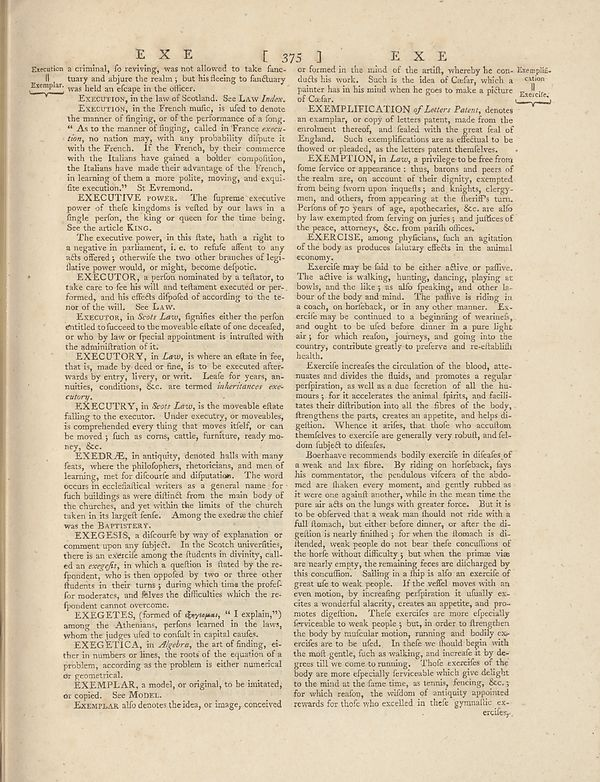
\includegraphics[width=0.85\textwidth]{../scans/page-1805-226885408318.jpg}
\caption*{Source scan: \texttt{page-1805-226885408318.jpg}}
\end{figure}

\end{document}
